\documentclass{article}
\usepackage{listings}
\usepackage{color}
\usepackage{amsmath}
\usepackage{amsfonts}
\usepackage{amssymb}
\usepackage{caption}
\usepackage{polski}
\usepackage{indentfirst}
\usepackage{graphicx}
\usepackage{pdfpages}
\usepackage{gauss}
\usepackage[section]{placeins}

\DeclareCaptionType{equ}[][List of equations]
\captionsetup[equ]{labelformat=empty}

%script adding bars in matrix
\usepackage{etoolbox}
\makeatletter
\patchcmd\g@matrix
 {\vbox\bgroup}
 {\vbox\bgroup\normalbaselines}% restore the standard baselineskip
 {}{}
\makeatother

\newcommand{\BAR}{%
  \hspace{-\arraycolsep}%
  \strut\vrule % the `\vrule` is as high and deep as a strut
  \hspace{-\arraycolsep}%
}
\definecolor{dkgreen}{rgb}{0,0.6,0}
\definecolor{gray}{rgb}{0.5,0.5,0.5}
\definecolor{mauve}{rgb}{0.58,0,0.82}

\lstset{frame=tb,
  language=Python,
  aboveskip=3mm,
  belowskip=3mm,
  showstringspaces=false,
  columns=flexible,
  basicstyle={\small\ttfamily},
  numbers=none,
  numberstyle=\tiny\color{gray},
  keywordstyle=\color{blue},
  commentstyle=\color{dkgreen},
  stringstyle=\color{mauve},
  breaklines=true,
  breakatwhitespace=true,
  tabsize=3,
  extendedchars=\true,
  inputencoding=utf8x,
}

\lstset{literate={ą}{{\k{a}}}1 {ł}{{\l{}}}1 {ń}{{\'n}}1 {ę}{{\k{e}}}1 {ś}{{\'s}}1 {ż}{{\.z}}1 {ó}{{\'o}}1 {ź}{{\'z}}1 {Ą}{{\k{A}}}1 {Ł}{{\L{}}}1 {Ń}{{\'N}}1 {Ę}{{\k{E}}}1 {Ś}{{\'S}}1 {Ż}{{\.Z}}1 {Ó}{{\'O}}1 {Ź}{{\'Z}}1 }

\begin{document}
\title{Sprawozdanie nr. 3 - Metody numeryczne i optymailzacja}
\author{Jakub Andryszczak 259519,\\ Jakub Żak 244255,\\ Maciej Cierpisz 249163}
\date{}
\maketitle

\newpage
\tableofcontents
%Tutaj zaczyna się wstęp

\newpage
\section{Zadanie nr. 1}
Znajdź „ręcznie” przybliżone rozwiązania w sensie kryterium najmniejszych kwadratów dla poniższych układów równań sprzecznych:

\begin{equation}
  (a)
  \begin{cases}
    3x_1-x_2=4 \\
    x_1+2x_2=0 \\
    2x_1+x_2=1
  \end{cases}\,
  (b)
  \begin{cases}
    3x_1+x_2+x_3=6 \\
    2x_1+3x_2 -x_3=1 \\
    2x_1-x_2+x_3=0\\
    3x_1-3x_2+3x_3=8\\
  \end{cases}\,.
\end{equation}
Przykład a:
\begin{equation}
  AX=B
\end{equation}


\begin{equation}
  A=
  \begin{gmatrix}[b]
   3 & -1 \\
   1 & 2 \\
   2 & 1 
  \end{gmatrix}
  B=
  \begin{gmatrix}[b]
    4\\0\\1
  \end{gmatrix}
\end{equation}

Obliczamy przybliżone wartości wektora X metodą najmniejszych kwadratów:

\begin{equation}
  X=(A^{T}A)^{-1} *(A^{T}B)
\end{equation}

\begin{equation}
  (A^{T}A)^{-1}=
  \linespread{2}\selectfont
  \addtolength{\arraycolsep}{1pt} 
  \begin{gmatrix}[b]
    \frac{6}{83} & -\frac{1}{83} \\
    -\frac{1}{83} & \frac{14}{83} 
  \end{gmatrix}
\end{equation}

\begin{equation}
  (A^{T}B)=
  \linespread{2}\selectfont
  \addtolength{\arraycolsep}{1pt} 
  \begin{gmatrix}[b]
    14 \\
    -3
  \end{gmatrix}
\end{equation}

\begin{equation}
  X=
  \linespread{2}\selectfont
  \addtolength{\arraycolsep}{1pt}
  \begin{gmatrix}[b]
    \frac{6}{83} & -\frac{1}{83} \\
    -\frac{1}{83} & \frac{14}{83} 
  \end{gmatrix}*
  \begin{gmatrix}[b]
    14 \\
    -3
  \end{gmatrix}=
  \begin{gmatrix}[b]
    \frac{87}{83} \\
    -\frac{56}{83} 
  \end{gmatrix}
\end{equation}

Przykład b:

\begin{equation}
  AX=B
\end{equation}


\begin{equation}
  A=
  \begin{gmatrix}[b]
   3 & 1 & 1 \\
   2 & 3 & -1\\
   2 & -1 & 1\\
   3 & -3 & 3  
  \end{gmatrix}
  B=
  \begin{gmatrix}[b]
    6\\1\\0\\8
  \end{gmatrix}
\end{equation}

Obliczamy przybliżone wartości wkektora X metodą najmniejszych kwadratów:

\begin{equation}
  X=(A^{T}A)^{-1} *(A^{T}B)
\end{equation}

\begin{equation}
  (A^{T}A)^{-1}=
  \linespread{2}\selectfont
  \addtolength{\arraycolsep}{1pt} 
  \begin{gmatrix}[b]
    \frac{2}{3} & -\frac{5}{6} & -\frac{3}{2} \\
    -\frac{5}{6} & \frac{7}{6} & 2 \\
    -\frac{3}{2} & 2 & \frac{43}{12} 
  \end{gmatrix}
\end{equation}

\begin{equation}
  (A^{T}B)=
  \linespread{2}\selectfont
  \addtolength{\arraycolsep}{1pt} 
  \begin{gmatrix}[b]
    44 \\
    -15\\
    29
  \end{gmatrix}
\end{equation}

\begin{equation}
  X=
  \linespread{2}\selectfont
  \addtolength{\arraycolsep}{1pt}
  \begin{gmatrix}[b]
    \frac{2}{3} & -\frac{5}{6} & -\frac{3}{2} \\
    -\frac{5}{6} & \frac{7}{6} & 2 \\
    -\frac{3}{2} & 2 & \frac{43}{12} 
  \end{gmatrix}*
  \begin{gmatrix}[b]
    44 \\
    -15\\
    29
  \end{gmatrix}=
  \begin{gmatrix}[b]
    -\frac{196}{71} \\
    \frac{293}{71} \\
    \frac{685}{71} 
  \end{gmatrix}
\end{equation}


\section{Zadanie nr. 2}
Znajdź parametry funkcji $ a_0+ a_1x^2 + a_2sin\frac{\pi*x}{2} $, która aproksymuje poniższy
zbiór punktów na płaszczyźnie w sensie kryterium najmniejszych kwadratów: (0,3), (1,0), (1,-1), (-1,2)\\

Poniżejimplementacja zadania w języku Python:

\begin{lstlisting}

  import numpy as np

  # Definicja wektorów y i x
  y = np.array([3, 0, -1, 2])
  x = np.array([0, 1, 1, -1])
  
  # Transpozycja dwóch wektorów
  y = y.reshape(-1, 1)
  x = x.reshape(-1, 1)
  
  # Tworzenie macierzy A
  A = np.hstack((np.ones_like(x), x**2, np.sin(np.pi * x / 2)))
  
  # Obliczenie z1
  z1 = np.linalg.inv(A.T @ A) @ A.T @ y
  
  print(z1)

\end{lstlisting}
\newpage

Otrzymane wartości współczynników a:

\begin{equation}
  \begin{cases}
    a_0=3\\
    a_1=-2,25\\
    a_2=-1,25
  \end{cases}
\end{equation}


\section{Zadanie nr. 3}
Pocisk jest wystrzeliwany z terytorium wroga, a jego położenie w locie jest obserwowane
przez radarowe urządzenia śledzące w następujących pozycjach:
\begin{figure}[h]
  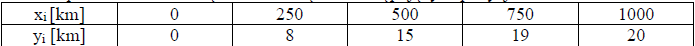
\includegraphics[scale=0.7]{tabelka.png}
  \centering
  \end{figure}

Załóżmy, że nasze źródła wywiadowcze wskazują, że wrogie pociski są zaprogramowane do
poruszania się po parabolicznym torze lotu. Oblicz jak daleko od punktu wystrzału spadnie
pocisk.

Z założeń wcześniej postawionych możemy wywnioskować że wzór dla danego pocisku będzie prezentować się następująco:
\begin{equation}
  y_i = ax_i^2 + bx_i + c
\end{equation}

Dla podanych wartości wyliczono macierz A:
\begin{equation}
  \begin{gmatrix}[b]
    0 & 0 & 1\\
    62500 & 250 & 1\\
    250000 & 500 & 1\\
    562500 & 750 & 1\\
    1000000 & 1000 & 1\\
  \end{gmatrix}
\end{equation}
Oraz wektor wynikowy:
\begin{equation}
  \begin{gmatrix}[b]
    0\\8\\15\\19\\20
  \end{gmatrix}
\end{equation}
Następnie wykonano kod w Python, który wyliczał współczynniki aproksymacji z podanych wartości:
\begin{lstlisting}
  import numpy as np

# Dane z radarów
xi = np.array([0, 250, 500, 750, 1000])
yi = np.array([0, 8, 15, 19, 20])

# Tworzenie macierzy A
A = np.vstack([xi**2, xi, np.ones(len(xi))]).T
print(A)
# Rozwiązanie równań normalnych
params = np.linalg.lstsq(A, yi, rcond=None)[0]

# Współczynniki aproksymacji
a, b, c = params
\end{lstlisting}
Wyniki obliczeń prezentują się następująco
\begin{equation}
  \begin{gmatrix}
    a=-1.94286*10^{-5}\\
    b=0.03982\\
    c=0.228571
  \end{gmatrix}
\end{equation}

Kolejno wyżej obliczone wartości podstawiono do wzoru na zasięg:
\begin{equation}
  Z = \frac{-b-(b^2-4ac)^{\frac{1}{2}}}{2a} = 2044.245[km]
\end{equation}

\section{Zadanie nr. 4}
Używając kryterium najmniejszych kwadratów dopasuj modele (a) i (b) do danych:
\begin{figure}[h]
  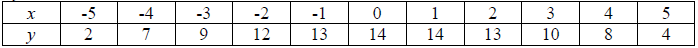
\includegraphics[scale=0.7]{tabelka_2.png}
  \centering
  \end{figure}

(a)
  \begin{equation}
y = a_0 + a_1x ,
\end{equation}\\

(b)
\begin{equation}
  y=a_0+a_1x+a_2x^2.
\end{equation}
Określ, który model lepiej dopasowuje się do danych na podstawie normy 2l błędu dopasowania:

Dla obu podpunktów wektor wynikowy wygląda tak samo
\begin{equation}
  b=
  \begin{gmatrix}[b]
  2\\7\\9\\12\\13\\14\\14\\13\\10\\8\\4  
  \end{gmatrix}
\end{equation}

Dla podpunktu a) macierz A prezentuje się następująco:
\begin{equation}
  A=
  \begin{gmatrix}[b]
    -5 & 1\\
    -4 & 1\\
    -3 & 1\\
    -2 & 1\\
    -1 & 1\\
    0 & 1\\
    1 & 1\\
    2 & 1\\
    3 & 1\\
    4 & 1\\
    5 & 1
  \end{gmatrix}
\end{equation}
Wykonano kod w Python który oblicza współczynniki oraz wyznacza normę 2l błędu dopasowania:
\begin{lstlisting}
  import numpy as np

# Dane
x = np.array([-5, -4, -3, -2, -1, 0, 1, 2, 3, 4, 5])
y = np.array([2, 7, 9, 12, 13, 14, 14, 13, 10, 8, 4])

# Model (a): y = ax + b
A_a = np.vstack([x, np.ones(len(x))]).T
print(A_a)
params_a = np.linalg.lstsq(A_a, y, rcond=None)[0]
a, b = params_a
y_pred_a = np.dot(A_a, params_a)
l2_error_a = np.linalg.norm(y - y_pred_a)
\end{lstlisting}
Współczynniki aproksymacji dla modelu (a):

a: 0.1818181818181818

b: 9.636363636363638
\newline Norma L2 błędu dopasowania dla modelu (a): 12.763584563479451
\newline

W przypadku podpunktu b) macierz A wynosi:
\begin{equation}
  A=
  \begin{gmatrix}[b]
    25 & -5 & 1\\
    16 & -4 & 1\\
    9 & -3 & 1\\
    4 & -2 & 1\\
    1 & -1 & 1\\
    0 & 0 & 1\\
    1 & 1 & 1\\
    4 & 2 & 1\\
    9 & 3 & 1\\
    16 & 4 & 1\\
    25 & 5 & 1
  \end{gmatrix}
\end{equation}
Kod do wyliczania współczynników i normy 2l:
\begin{lstlisting}
  A_b = np.vstack([x**2, x, np.ones(len(x))]).T
print(A_b)
params_b = np.linalg.lstsq(A_b, y, rcond=None)[0]
y_pred_b = np.dot(A_b, params_b)
l2_error_b = np.linalg.norm(y - y_pred_b)
print("Współczynniki aproksymacji dla modelu (b):")
print("a:", params_b[0])
print("b:", params_b[1])
print("c:", params_b[2])
print("Norma L2 błędu dopasowania dla modelu (b):", l2_error_b)
\end{lstlisting}
Współczynniki aproksymacji dla modelu (b):

a: -0.4335664335664337

b: 0.18181818181818166

c: 13.972027972027968
\newline Norma L2 błędu dopasowania dla modelu (b): 1.2737258819611161
\newline

Model (b) lepiej dopasowuje się do danych.
\newpage
\section{Zadanie nr. 5}

Dopasuj szereg funkcji kosinusowych $ g(x) = \sum_{j=0}^{n} c_j cos jx $ do funkcji kwadratowej
$ f(x)=\pi^2-x^2 $ w taki sposób, aby minimalizować błąd: $ ||f(x) - g(x)||_2  $ wprzedziale $[0, \pi]$
Oceń błąd dla n = 1, 2, 3, ..., 10.\\

Poniżej implementacja rozwiązania w języku Python:

\begin{lstlisting}
  import numpy as np
  import matplotlib.pyplot as plt
  
  # Funkcja f(x)
  def f(x):
    return np.pi**2 - x**2
  
  # Funkcja g(x)
  def g(x, n, c):
    sum = 0
    for j in range(n+1):
      sum += c[j] * np.cos(j*x)
    return sum
  
  # Minimalizacja bledu
  def minimize_error(n):
    # Wspolczynniki c
    c = np.zeros(n+1)
  
    # Macierz A
    A = np.zeros((n+1, n+1))
    for i in range(n+1):
      for j in range(n+1):
        A[i, j] = np.cos(i*j)
  
    # Wektor b
    b = np.zeros(n+1)
    for i in range(n+1):
      b[i] = f(i*np.pi/n)
  
    # Rozwiązanie ukladu równań
    c = np.linalg.solve(A, b)
  
    # Obliczenie bledu
    error = 0
    for i in range(n+1):
      error += (f(i*np.pi/n) - g(i*np.pi/n, n, c))**2
  
    return error
  
  for n in range(1, 11):
    # Wspolczynniki c
    c = np.zeros(n+1)
  
    # Macierz A
    A = np.zeros((n+1, n+1))
    for i in range(n+1):
      for j in range(n+1):
        A[i, j] = np.cos(i*j)
  
    # Wektor b
    b = np.zeros(n+1)
    for i in range(n+1):
      b[i] = f(i*np.pi/n)
  
    # Rozwiązanie układu równań
    c = np.linalg.solve(A, b)
  
  
  # Bledy
  for n in range(1, 11):
    error = minimize_error(n)
    print(f"n={n}, błąd={error}")
   
\end{lstlisting}

Wyniki obliczeń błędów dla zadanych wartości n:
\begin{figure}[h]
  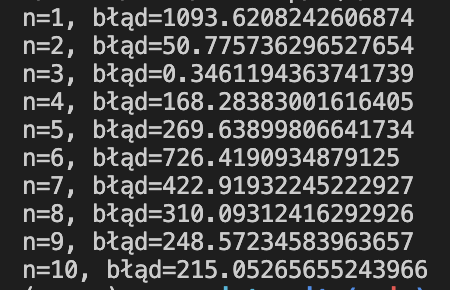
\includegraphics[scale=0.7]{bledy5.png}
  \centering
  \end{figure}
\newpage

\section{Zadanie nr. 6}
Dla macierzy  

\[ A = \begin{pmatrix}  

1 & 2 & 3 \\ 

4 & 5 & 6 \\ 

7 & 8 & 9 \\ 

10 & 11 & 12 \\ 

13 & 14 & 15 \\ 

\end{pmatrix} \] 
Oraz dokładnego rozwiązania 
\[ x = \begin{pmatrix}  

1 \\ 

2 \\ 

3 \\ 

\end{pmatrix} \] 
wyznacz wektor danych dla modelu: Ax=b, a następnie:

(a) dla N = 10, wyznacz błąd rozwiązania $||x-x_*||$ oraz błąd residualny $||b-Ax||_2$ w funkcji parametru regularyzacji stosując: (i) standardową regularyzację Tichnowa,
(ii) TSVD.

(b) oszacuj rank(A) i cond(A) oraz $A^+$,

(c) wyznacz krzywą L i oszacuj optymalną wartość parametru regularyzacji dla obu metod.




Napisano skrypt: 

 

\begin{lstlisting} 

import numpy as np 

Import matplotlib.pyplot 

  

A = np.array([ [1, 2, 3], 

                          [4, 5, 6], 

                          [7, 8, 9], 

                          [10, 11, 12] 

                          [13, 14, 15]) 

x= np.array([1, 2, 3]).transpose() 

 

#Obliczenie wartosci wektora B 

B = np.dot(A, x) 

Pseudo_inv_A = np.linalg.pinv(A) 

 

#Obliczenie wskaźnika uwarunkowania macierzy A 

cond_A = np.linalg.cond(A) 

 

#Wyznaczenie rzedu macierzy A 

Rank_A = round(np.linalg.matrix_rank(A), 0) 

x0 = np.dot(pseudo_inv_A, B) 

 

#Obliczenie wartosci bledów 

U, S, Vt = np.linalg.svd(A, full_matrices=False) 

y1 = np.matmul(U.T, B) 

S_inv = np.diag(1/S) 

y2 = np. Matmul(S_inv, y1) 

x1 = np.matmul(Vt.T, y2) 

  

#Obliczenie wartosci bledu rozwiązania 

blad_rozw = np.linalg.norm(x0 – x1, ord=2) 

 

#Obliczenie wartosci bledu residualnego 

blad_resi = np.linalg.norm(B – x1.dot(pseudo_inv_A), ord=2) 

 

#Regularyzacja Tichnowa 

L = np.linsapce(0.00001, 1 , 5) 

blad_tich = np. Zeros(5) 

X_tich = np.zeros(5) 

For i in range(len(L)): 
	x_tich[i] = np.linalg.norm(x1.dot(np.linalg.pinv(A)) - B, ord=2) + L[i] 
	blad=tich[i] = np.linalg.norm(x1 – x_tich[i]) 

 

 \end{lstlisting} 

 

Otrzymano następujące wartości: 

Błąd rozwiązania: 1.368774871883577e-15 

Błąd residualny: 123.349910 

Błąd regularyzacji Tichnowa: 215.385005 

Cond(A): 3.5681136352506475e+16 

Rank(A): 2 

Krzywa L: 
\begin{figure}[h]
  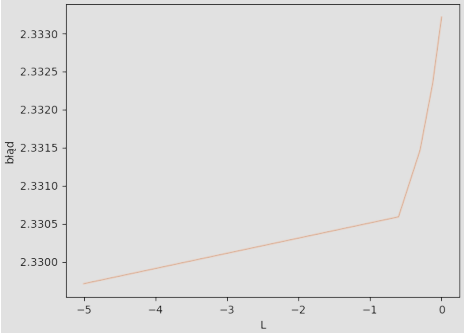
\includegraphics[scale=0.7]{Krzywa_L.png}
  \centering
  \end{figure}

\section{Zadanie nr. 7}
Niech c = [0 1 ... N-1$]^T$ należy do $ R^N$ będzie pierwszą kolumną, a

r=[0 -1 ... -N+1] należy do $ R^N$ pierwszym wierszem macierzy Toeplitza.

Niech:

(A) x*=[1 2 ... N$]^T$ należy do $ R^N$,

(B) $x*~N(0,1)$ należy do $R^N$ (rozkład normalny).

Wykonaj projekcję “w przód” obu rozwiązań: $Ax*=b$ , a następnie:

(a) dla N = 10, wyznacz błąd rozwiązania $||x-x_*||$ oraz błąd residualny 

$||b-Ax||_2$ w funkcji parametru regularyzacji stosując: (i) standardową regularyzację Tichnowa,
(ii) TSVD.

(b) dla N = 10 przedstaw krzywe L, oddzielnie dla danych (A) i (B).

(c) oszacuj rank(A) i cond(A) dla N = 5, 10, 50, 100.

(d) przedstaw wykres zależności optymalnego parametru regularyzacji w funkcji wymiaru
N dla danych (A) i (B),

(e) Uzasadnij dlaczego błąd rozwiązania jest dużo mniejszy dla danych typu (A) niż dla
danych (B).\\

Ponizej kod realizujacy zadanie:

\begin{lstlisting}
import numpy as np
import matplotlib.pyplot as plt
from scipy.linalg import toeplitz

def multiply_matrix_vector(A, x):
    return A.dot(x)

def calculate_errors(x_approx, x_exact, A, b):
    solution_error = np.linalg.norm(x_approx - x_exact)
    residual_error = np.linalg.norm(b - A.dot(x_approx))
    return solution_error, residual_error

def perform_regularizations(A, b, x_exact, lambda_tikhonov, k_tsvd):
    # Tikhonov Regularization
    A_tilde = np.vstack((A, lambda_tikhonov * np.eye(A.shape[1])))
    b_tilde = np.concatenate((b, np.zeros(A.shape[1])))
    x_tikhonov = np.linalg.lstsq(A_tilde, b_tilde, rcond=None)[0]

    # TSVD Regularization
    U, sigma, VT = np.linalg.svd(A, full_matrices=False)
    sigma_truncated = np.zeros_like(sigma)
    sigma_truncated[:k_tsvd] = sigma[:k_tsvd]
    Sigma_truncated = np.diag(sigma_truncated)
    Sigma_truncated_inv = np.diag([1 / s if s > 0 else 0 for s in sigma_truncated])
    x_tsvd = VT.T @ Sigma_truncated_inv @ U.T @ b

    # Calculate and store errors
    solution_error, residual_error = calculate_errors(x_tikhonov, x_exact, A, b)

    return x_tikhonov, solution_error, residual_error

def estimate_rank_and_condition(A):
    rank_A = np.linalg.matrix_rank(A)
    cond_A = np.linalg.cond(A)
    return rank_A, cond_A

def plot_l_curve(A, b, x_exact, lambda_values, subplot_title):
    norms_solution = []
    norms_residual = []

    for lam in lambda_values:
        _, solution_error, residual_error = perform_regularizations(A, b, x_exact, lam, N)
        norms_solution.append(solution_error)
        norms_residual.append(residual_error)

    plt.loglog(norms_residual, norms_solution, label=subplot_title)
    plt.xlabel('Norma resztowa ||Ax-b||')
    plt.ylabel('Norma rozwiązania ||x-x*||')
    plt.grid(True)

def plot_l_curve_tsvd(A, b, x_exact, k_values, dataset_name):
    norms_solution = []
    norms_residual = []

    U, S, Vt = np.linalg.svd(A, full_matrices=False)

    for k in k_values:
        S_truncated = np.zeros_like(S)
        S_truncated[:k] = S[:k]
        Sigma_truncated_inv = np.diag(1 / S_truncated[:k])
        x_tsvd = Vt[:k, :].T @ Sigma_truncated_inv @ U[:, :k].T @ b

        solution_error, residual_error = calculate_errors(x_tsvd, x_exact, A, b)
        norms_solution.append(solution_error)
        norms_residual.append(residual_error)

    plt.loglog(norms_residual, norms_solution, label=f'TSVD for {dataset_name}')
    plt.xlabel('Norma resztowa (||Ax - b||)')
    plt.ylabel('Norma rozwiązania (||x-x*||)')
    plt.grid(True)

def plot_optimal_regularization_parameter(N_values):
    optimal_lambda_A = []
    optimal_lambda_B = []

    for N in N_values:
        # Generate Toeplitz matrix A
        c = np.arange(N)
        r = np.concatenate(([c[0]], -c[1:]))
        A = toeplitz(c, r)

        # Generate solutions x* for datasets (A) and (B)
        x_star_a = np.arange(1, N + 1)
        x_star_b = np.random.normal(0, 1, N)

        # Generate forward projections b for datasets (A) and (B)
        b_a = multiply_matrix_vector(A, x_star_a)
        b_b = multiply_matrix_vector(A, x_star_b)

        # Determine optimal lambda for dataset (A) - Placeholder
        optimal_lambda_A.append(np.argmin(
            [calculate_errors(perform_regularizations(A, b_a, x_star_a, lam, N)[0], x_star_a, A, b_a)[1] for lam in
             lambda_values]))

        # Determine optimal lambda for dataset (B) - Placeholder
        optimal_lambda_B.append(np.argmin(
            [calculate_errors(perform_regularizations(A, b_b, x_star_b, lam, N)[0], x_star_b, A, b_b)[1] for lam in
             lambda_values]))

    # Plotting the optimal lambda values
    plt.figure(figsize=(10, 6))
    plt.plot(N_values, optimal_lambda_A, 'o-', label='Optymalna wartość lambda dla zbioru danych (A)')
    plt.plot(N_values, optimal_lambda_B, 's-', label='Optymalna wartość lambda dla zbioru danych(B)')
    plt.xlabel('Wielkość macierzy N')
    plt.ylabel('Optymalna wartość parametru lambda')
    plt.title('Optymalna wartość parametru lambda w zależności od wielkości macierzy N')
    plt.legend()
    plt.grid(True)
    plt.tight_layout()
    plt.show()

# Main code section
lambda_values = np.logspace(-15, 1, 100)
N_values = [5, 10, 50, 100]

# Estimate and print rank and condition number for Toeplitz matrices of different sizes
for N in N_values:
    c = np.arange(N)
    r = np.concatenate(([c[0]], -c[1:]))
    A = toeplitz(c, r)
    rank_A, cond_A = estimate_rank_and_condition(A)
    print(f"N={N}: rank(A)={rank_A}, cond(A)={cond_A:.2e}")

# Create plots for the L-curve for data set (A) and (B) for N=10
N = 10
c = np.arange(N)
r = np.concatenate(([c[0]], -c[1:]))
A = toeplitz(c, r)

# Generate solutions x* for datasets (A) and (B)
x_star_a = np.arange(1, N + 1)
x_star_b = np.random.normal(0, 1, N)

# Forward projections b
b_a = multiply_matrix_vector(A, x_star_a)
b_b = multiply_matrix_vector(A, x_star_b)

k_values = range(1, min(A.shape) + 1)

plt.figure(figsize=(12, 6))

# Plot the L-curve for data set (A)
plt.subplot(1, 2, 1)
plot_l_curve(A, b_a, x_star_a, lambda_values, 'Zbiór danych (A)')

# Plot the L-curve for data set (B)
plt.subplot(1, 2, 2)
plot_l_curve(A, b_b, x_star_b, lambda_values, 'Zbiór danych (B)')

plt.suptitle('Krzywa L dla Regularyzacji Tichnowa')
plt.legend()
plt.tight_layout()
plt.show()

plt.figure(figsize=(12, 6))

# Plot the L-curve for data set (A)
plt.subplot(1, 2, 1)
plot_l_curve_tsvd(A, b_a, x_star_a, k_values, 'Zbiór danych (A)')

# Plot the L-curve for data set (B)
plt.subplot(1, 2, 2)
plot_l_curve_tsvd(A, b_b, x_star_b, k_values, 'Zbiór danych (B)')

plt.suptitle('Krzywa L dla Regularyzacji TSVD')
plt.legend()
plt.tight_layout()
plt.show()

# Plot optimal regularization parameter as a function of N for datasets (A) and (B)
plot_optimal_regularization_parameter(N_values)

\end{lstlisting}

\begin{figure}[!h]
  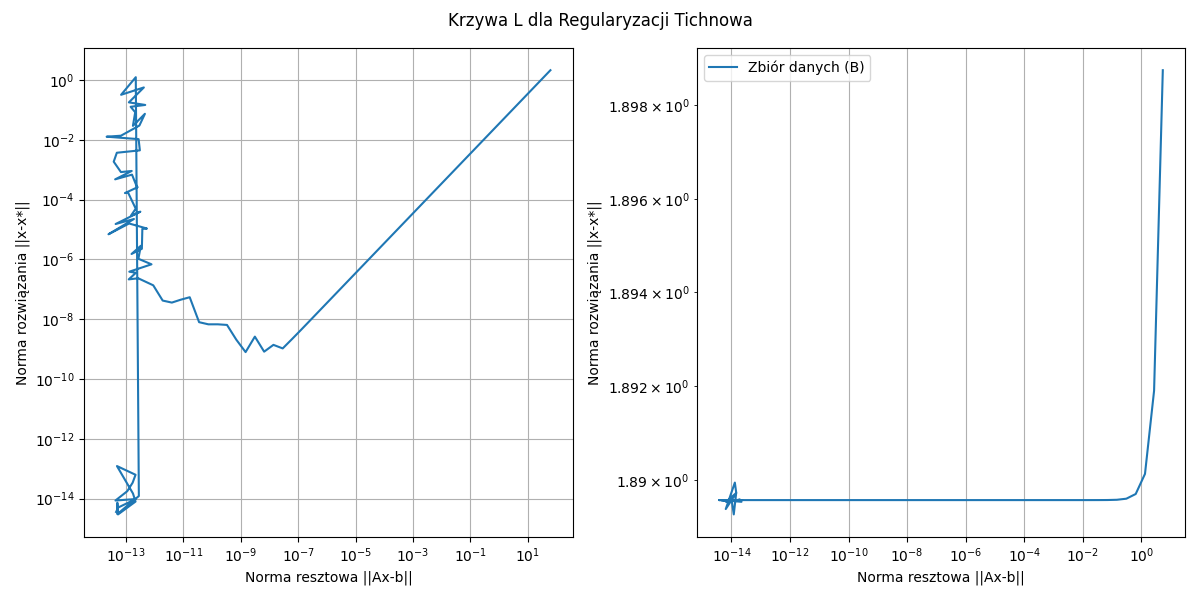
\includegraphics[scale=0.45]{Ltikhonov.png}
  \centering
  \end{figure}
  \begin{figure}[!h]
    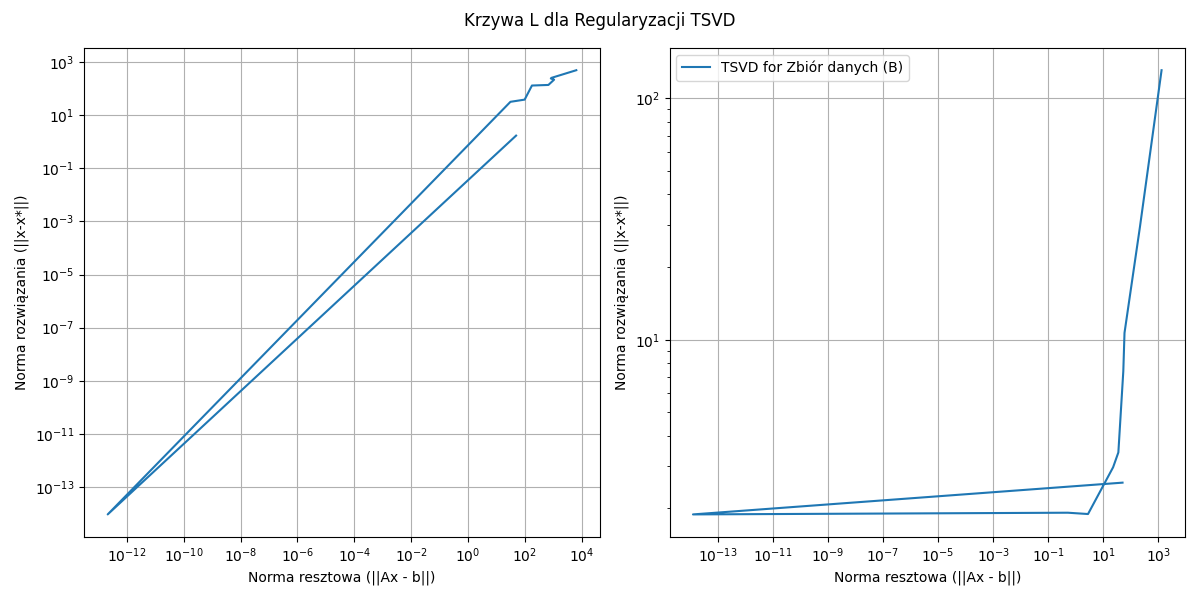
\includegraphics[scale=0.45]{LTSVD.png}
    \centering
    \end{figure}
    \begin{figure}[!h]
      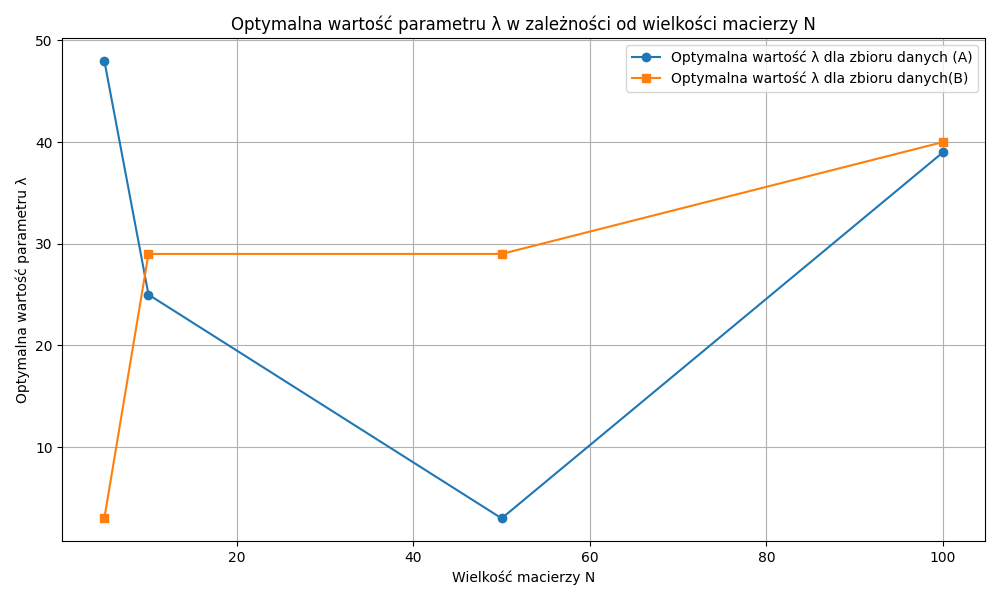
\includegraphics[scale=0.55]{optimals.png}
      \centering
      \end{figure}
Wyniki obliczeń szacunkowych:
      \begin{equation}
        \begin{cases}
          N=5 : rank(A) = 2 , cond(A) = 3.40e17\\
          N=10 : rank(A) = 2 , cond(A) = 2.03e18\\
          N=50 : rank(A) = 2 , cond(A) = 6.36e19\\
          N=100 : rank(A) = 2 , cond(A) = 6.49e20\\
      
      
        \end{cases}
      \end{equation}
\section{Wnioski}
Bląd rozwiązania dla danych typu A jest duzo mniejszy ze wzgledu na wykorzystanie w zbiorze B liczb z zakresu rozkładu normalnego.\\



\end{document} 